%advantages
A major advantage of anonymous usage data is the fact that it captures developers in their natural habitat, without any observational bias. Deriving conclusions from hours of developers' field work is naturally more convincing than from hour-long, in-lab developer studies. One type of questions that usage data is well-suited to answer uses measurement of the magnitude of occurrence of a specific event. For instance, researchers may want to know ``How often do developers invoke the pull-up refactoring'' or ``How often is the file search invoked?''. By performing a count of a specific message in the collected logs, researchers can easily calculate frequencies of specific actions that can be often sufficient to answer important research questions. 

%disadvantages
However, researchers must be wary of a few common issues with magnitude analysis. First, in any sufficiently large set of user logs there is a small set of developers that will use the feature/tool under analysis orders of magnitude more often than the general population, potentially skewing the data. 
Second, attempts to attribute time to individual activities are fraught with difficulties. For instance, there is a temptation to report the percentage of time spent doing activity X. Yet, because the data is based on a stream of activities any time calculation requires making unsound assumptions on what happens in between these events.

%example
Murphy et al's work on understanding Eclipse IDE usage provides several examples of magnitude analysis being used effectively. By simply counting instances of events in developers' activity streams they were able to present how often developers accessed certain views, the top 10 commands executed by developers, and the percentage of developers that used each specific refactoring command. In spite of the simplicity of this analysis its ideal for identifying heavily used features for improvements and unused features for removal, as well as for getting a sense of how developers are currently working. 


\begin{figure}
  \centering
  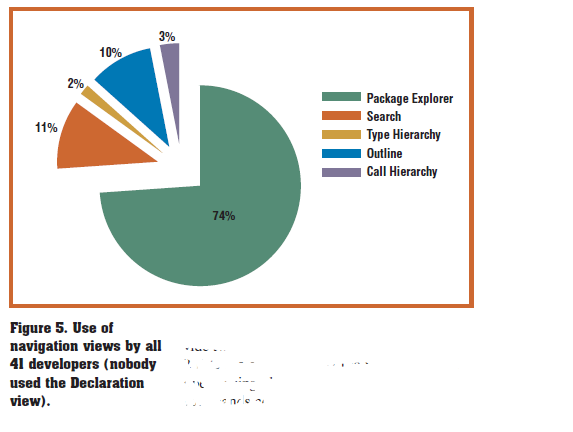
\includegraphics{eclipse}
  \caption{Breakdown of Navigation-Focused View Usage in Eclipse}\label{fig:eclipse}
\end{figure}


